%%%%%%%%%%%%%%%%%%%%%%%%%%%%%%%%%%%%%%%%%%%%%%%
%%%     Declarations (skip to Begin Document, line 101, for parts you fill in)
%%%%%%%%%%%%%%%%%%%%%%%%%%%%%%%%%%%%%%%%%%%%%%%

\documentclass[10pt]{article}

\usepackage{geometry}  % Lots of layout options.  See http://en.wikibooks.org/wiki/LaTeX/Page_Layout
\geometry{letterpaper}  % ... or a4paper or a5paper or ... 
\usepackage{fullpage}  % somewhat standardized smaller margins (around an inch)
\usepackage{setspace}  % control line spacing in latex documents
\usepackage[parfill]{parskip}  % Activate to begin paragraphs with an empty line rather than an indent

\usepackage{url}

\usepackage{amsmath,amssymb}  % latex math
\usepackage{empheq} % http://www.ctan.org/pkg/empheq
\usepackage{bm,upgreek}  % allows you to write bold greek letters (upper & lower case)

% allows strikethroughs in math via \cancel{math text goes here}
\usepackage{cancel}

% provides adjustwidth environment to temporarily change margins
% \begin{adjustwidth}{left change length}{\right change length}
\usepackage{changepage}

% for typsetting algorithm pseudocode see http://en.wikibooks.org/wiki/LaTeX/Algorithms_and_Pseudocode
\usepackage{algorithmic,algorithm}  

\usepackage{graphicx}  % inclusion of graphics; see: http://en.wikibooks.org/wiki/LaTeX/Importing_Graphics
% allow easy inclusion of .tif, .png graphics
\DeclareGraphicsRule{.tif}{png}{.png}{`convert #1 `dirname #1`/`basename #1 .tif`.png}

\usepackage{subfigure}  % allows subfigures in figure
%\usepackage{caption}
%\usepackage{subcaption}

\usepackage{xspace}
\newcommand{\latex}{\LaTeX\xspace}

\usepackage{color}  % http://en.wikibooks.org/wiki/LaTeX/Colors

\long\def\ans#1{{\color{blue}{\em #1}}}
\long\def\ansnem#1{{\color{blue}#1}}
\long\def\boldred#1{{\color{red}{\bf #1}}}
\long\def\boldred#1{\textcolor{red}{\bf #1}}
\long\def\boldblue#1{\textcolor{blue}{\bf #1}}
\long\def\todo#1{\textcolor{red}{\bf TODO: #1}}

% misc math defs
\newcommand{\norm}[1]{\left\lVert#1\right\rVert}

% Useful package for syntax highlighting of specific code (such as python) -- see below
\usepackage{listings}  % http://en.wikibooks.org/wiki/LaTeX/Packages/Listings
\usepackage{textcomp}

%%% The following lines set up using the listings package
\renewcommand{\lstlistlistingname}{Code Listings}
\renewcommand{\lstlistingname}{Code Listing}

%%% Specific for python listings
\definecolor{gray}{gray}{0.5}
\definecolor{green}{rgb}{0,0.5,0}

\lstnewenvironment{python}[1][]{
\lstset{
language=python,
basicstyle=\footnotesize,  % could also use this -- a little larger \ttfamily\small\setstretch{1},
stringstyle=\color{red},
showstringspaces=false,
alsoletter={1234567890},
otherkeywords={\ , \}, \{},
keywordstyle=\color{blue},
emph={access,and,break,class,continue,def,del,elif ,else,%
except,exec,finally,for,from,global,if,import,in,i s,%
lambda,not,or,pass,print,raise,return,try,while},
emphstyle=\color{black}\bfseries,
emph={[2]True, False, None, self},
emphstyle=[2]\color{green},
emph={[3]from, import, as},
emphstyle=[3]\color{blue},
upquote=true,
morecomment=[s]{"""}{"""},
commentstyle=\color{gray}\slshape,
emph={[4]1, 2, 3, 4, 5, 6, 7, 8, 9, 0},
emphstyle=[4]\color{blue},
literate=*{:}{{\textcolor{blue}:}}{1}%
{=}{{\textcolor{blue}=}}{1}%
{-}{{\textcolor{blue}-}}{1}%
{+}{{\textcolor{blue}+}}{1}%
{*}{{\textcolor{blue}*}}{1}%
{!}{{\textcolor{blue}!}}{1}%
{(}{{\textcolor{blue}(}}{1}%
{)}{{\textcolor{blue})}}{1}%
{[}{{\textcolor{blue}[}}{1}%
{]}{{\textcolor{blue}]}}{1}%
{<}{{\textcolor{blue}<}}{1}%
{>}{{\textcolor{blue}>}}{1},%
%framexleftmargin=1mm, framextopmargin=1mm, frame=shadowbox, rulesepcolor=\color{blue},#1
framexleftmargin=1mm, framextopmargin=1mm, frame=single,#1
}}{}
%%% End python code listing definitions

\DeclareMathOperator{\diag}{diag}
\DeclareMathOperator{\cov}{cov}

%%%%%%%%%%%%%%%%%%%%%%%%%%%%%%%%%%%%%%%%%%%%%%%
%%%     Begin Document
%%%%%%%%%%%%%%%%%%%%%%%%%%%%%%%%%%%%%%%%%%%%%%%

\begin{document}

\begin{center}
    {\Large {\bf ISTA 421 / INFO 521 - Homework 1}} \\
\end{center}

\begin{flushright}
Charles Kenneth "Ken" Youens-Clark

Graduate 
\end{flushright}

\vspace{1cm}

\emph{Note: I discussed problems 3-5 with TA Farig Sadeque and students Matthew Miller and Kai Blumberg.}

\begin{enumerate}

%%%   Problem 1
\item \label{prob:1} [0 points]
Python setup.

%%%   Problem 2
\item \label{prob:2} [1 point]
{\bf Exercise 1.1} from FCMA p.35

\begin{figure}[htb]
\begin{center}
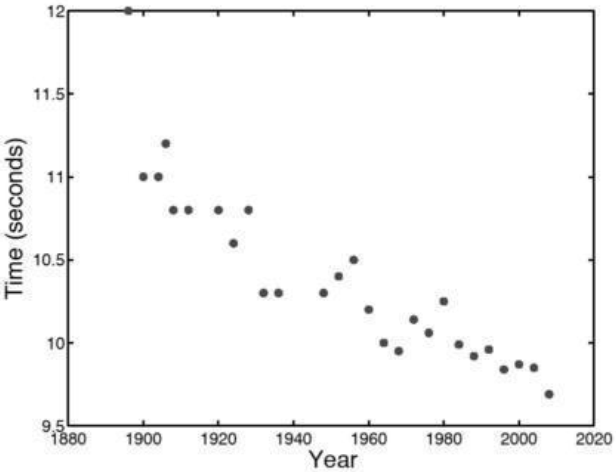
\includegraphics[width=6cm]{figures/figure1-1_p2}
\caption{Reproduction of figure 1.1, Olympic men's 100m data}
\end{center}
\end{figure}
By examining Figure 1.1 [from p. 2 of FCMA, reproduced here], estimate (by hand / in your head) the kind of values we should expect for $w_0$ (y-intercept) and $w_1$ (slope) as parameters of a line fit to the data (e.g., High? Low?  Positive?  Negative?).  (No computer or calculator calculation is needed here -- just estimate!)

{\bf Solution.} 

I added a red line to the image above to indicate the kind of slope I would expect. Y intercept would be around 11.25, slope drops about 0.5 seconds every 20 years, so -20/0.5 = -40.


%%%   Problem 3
\item \label{prob:3} [2 points]
{\bf Exercise 1.3} from FCMA p.35

Show that:
\begin{eqnarray*}
\mathbf{w}^\top\mathbf{X}^\top\mathbf{X}\mathbf{w} = w_0^2 \left( \sum_{n=1}^N x_{n1}^2 \right) + 2w_0w_1 \left( \sum_{n=1}^N x_{n1}x_{n2} \right) + w_1^2 \left( \sum_{n=1}^N x_{n2}^2 \right),
\end{eqnarray*}
where
\begin{eqnarray*}
\mathbf{w} = 
    \begin{bmatrix}
    w_0 \\[0.3em]
    w_1
    \end{bmatrix}
    ,
\mathbf{X} = 
    \begin{bmatrix}
    x_{11} & x_{12} \\[0.3em]
    x_{21} & x_{22} \\[0.3em]
    x_{31} & x_{32} \\[0.3em]
    \vdots & \vdots \\[0.3em]
    x_{N1} & x_{N2}
    \end{bmatrix}
    .
\end{eqnarray*}

{\bf Solution.}

\begin{eqnarray*}
\mathbf{X}^\top = 
    \begin{bmatrix}
    x_{11} & x_{12} & x_{13} & \dots & x_{1n} \\[0.3em]
    x_{12} & x_{22} & x_{32} & \dots & x_{n2} \\[0.3em]
    \end{bmatrix}
\end{eqnarray*}


\begin{eqnarray*}
\mathbf{X}^\top\mathbf{X} = 
    \begin{bmatrix}
    {\sum_{n=1}^N x_{n1}^2}      & {\sum_{n=1}^N x_{n1} x_{n2}} \\[0.3em]
    {\sum_{n=1}^N x_{n2} x_{n1}} & {\sum_{n=1}^N x_{n2}^2}      \\[0.3em]
    \end{bmatrix}
\end{eqnarray*}

\begin{eqnarray*}
\mathbf{w}^\top = 
    \begin{bmatrix}
    w_0 & w_1 \\[0.3em]
    \end{bmatrix}
\end{eqnarray*}


\begin{eqnarray*}
\mathbf{w}^\top\mathbf{X}^\top\mathbf{X} = 
	\begin{bmatrix}
	w_0{\sum_{n=1}^N x_{n1}^2} + w_1{\sum_{n=1}^N x_{n2} x_{n1}} & 
	w_0{\sum_{n=1}^N x_{n1} x_{n2} + w_{\sum_{n=1}^N x_{n2}^2}}
	\end{bmatrix}
\end{eqnarray*}

\begin{eqnarray*}
\mathbf{w} = 
    \begin{bmatrix}
    w_0 \\[0.3em]
    w_1
    \end{bmatrix}
\end{eqnarray*}    

\begin{eqnarray*}
\mathbf{w}^\top\mathbf{X}^\top\mathbf{X}\mathbf{w}  = 
	w_0^2   \left( {\sum_{n=1}^N x_{n1}^2}      \right) + 
	w_0 w_1 \left( {\sum_{n=1}^N x_{n2} x_{n1}} \right) + 
	w_0 w_1 \left( {\sum_{n=1}^N x_{n1} x_{n2}} \right) + 
	w_1^2   \left( {\sum_{n=1}^N x_{n2}^2}      \right)
\end{eqnarray*}

\begin{eqnarray*}
\mathbf{w}^\top\mathbf{X}^\top\mathbf{X}\mathbf{w}  = 
	w_0^2 \left( {\sum_{n=1}^N x_{n1}^2} \right) + 
	2w_0 w_1 \left( {\sum_{n=1}^N x_{n1} x_{n2}} \right) + 
	w_1^2 \left( {\sum_{n=1}^N x_{n2}^2} \right)
\end{eqnarray*}


%%%   Problem 4
\item \label{prob:4} [1 point]
{\bf Exercise 1.4} from FCMA p.35

Using $\mathbf{w}$ and $\mathbf{X}$ as defined in the previous exercise, show that ${(\mathbf{X}\mathbf{w})}^\top = {\mathbf{w}}^\top{\mathbf{X}}^\top$ by multiplying out both sides.

{\bf Solution.} 

Given:

\begin{eqnarray*}
	\mathbf{X} = 
    \begin{bmatrix}
    x_{11} & x_{12} \\[0.3em]
    x_{21} & x_{22} \\[0.3em]
    x_{31} & x_{32} \\[0.3em]
    \vdots & \vdots \\[0.3em]
    x_{N1} & x_{N2}
    \end{bmatrix}
    ,
    \mathbf{w} = 
    \begin{bmatrix}
    w_0 \\[0.3em]
    w_1
    \end{bmatrix}
\end{eqnarray*}

Then:

\begin{eqnarray*}
\begin{aligned}
    \mathbf{Xw} &=
    \begin{bmatrix} 
    x_{11} w_0 + x_{12} w_1 \\
    x_{21} w_0 + x_{22} w_1 \\
    x_{31} w_0 + x_{32} w_1 \\
    \dots \\
    x_{N1} w_0 + x_{N2} w_1 \\
    \end{bmatrix} 
    \\
    (\mathbf{Xw})^\top &=
    \begin{bmatrix} 
    x_{11} w_0 + x_{12} w_1 &
    x_{21} w_0 + x_{22} w_1 &
    x_{31} w_0 + x_{32} w_1 &
    \dots &
    x_{N1} w_0 + x_{N2} w_1 
    \end{bmatrix} 
\end{aligned}
\end{eqnarray*}

Given:

\begin{eqnarray*}   
	\mathbf{w}^\top = \begin{bmatrix} w_0 & w_1 \end{bmatrix}
	,
    \mathbf{X}^\top = 
    \begin{bmatrix}
    x_{11} & x_{21} & x_{31} & \dots & x_{N1} \\[0.3em]
    x_{12} & x_{22} & x_{32} & \dots & x_{N2} \\[0.3em]
    \end{bmatrix}
\end{eqnarray*}

Then:

\begin{eqnarray*}
    \mathbf{w}^\top \mathbf{X}^\top = 
    \begin{bmatrix} 
    w_0 x_{11} + w_1 x_{12} &
    w_0 x_{21} + w_1 x_{22} &
    w_0 x_{31} + w_1 x_{32} &
    \dots &
    w_0 x_{N1} + w_1 x_{N2} &
    \end{bmatrix}
\end{eqnarray*}

Therefore ${(\mathbf{X}\mathbf{w})}^\top = {\mathbf{w}}^\top{\mathbf{X}}^\top$

%%%   Problem 5
\item \label{prob:5} [2 points]
{\bf Exercise 1.5} from FCMA p.35  % [1pt]

When multiplying a scalar by a vector (or matrix), we multiply each element of the vector (or matrix) by that scalar.  For $\mathbf{x}_n = {[ x_{n1}, x_{n2} ]}^\top$, $\mathbf{t} = {[ t_1,...,t_N ]}^\top$, $\mathbf{w} = {[ w_0, w_1 ]}^\top$, and
\begin{eqnarray*}
\mathbf{X} = 
    \begin{bmatrix}
    {\mathbf{x}_{1}}^\top \\[0.3em]
    {\mathbf{x}_{2}}^\top \\[0.3em]
    \vdots \\[0.3em]
    {\mathbf{x}_{N}}^\top
    \end{bmatrix}
\end{eqnarray*}
show that
\begin{eqnarray*}
\sum_{n} \mathbf{x}_n t_n = \mathbf{X}^\top\mathbf{t}
\end{eqnarray*}
and
\begin{eqnarray*}
\sum_{n} \mathbf{x}_n \mathbf{x}_n ^\top \mathbf{w} = \mathbf{X}^\top\mathbf{X} \mathbf{w}
\end{eqnarray*}

{\bf Solution Part 1}

Given: 
\begin{eqnarray*}
\begin{aligned}
	\mathbf{t} &=
	\begin{bmatrix}
	t_1 \\
	t_2 \\
	\vdots \\
	t_n
	\end{bmatrix}
	\\
	\mathbf{X}^\top &= \begin{bmatrix} \mathbf{x}_1 & \mathbf{x}_2 & \mathbf{x}_3 & \dots & \mathbf{x}_N \end{bmatrix}
	\\
	\mathbf{X}^\top\mathbf{t} &= \mathbf{x}_1 t_1 + \mathbf{x}_2 t_2 + \mathbf{x}_3 t_3 \dots \mathbf{x}_N t_N
	\\
	&= \sum_n \mathbf{x}_n t_n
\end{aligned}
\end{eqnarray*}

{\bf Solution Part 2}

\begin{eqnarray*}
\sum_{n} \mathbf{x}_n \mathbf{x}_n ^\top \mathbf{w} = \mathbf{X}^\top\mathbf{X} \mathbf{w}
\end{eqnarray*}

Divide both sides by $\mathbf{w}$:

\begin{eqnarray*}
\sum_{n} \mathbf{x}_n \mathbf{x}_n ^\top = \mathbf{X}^\top\mathbf{X}
\end{eqnarray*}

Solve the right side given:

\begin{eqnarray*}
\begin{aligned}
    \mathbf{X} &= 
        \begin{bmatrix}
        {\mathbf{x}_{1}}^\top \\
        {\mathbf{x}_{2}}^\top \\
        {\mathbf{x}_{3}}^\top \\
        \vdots \\
        {\mathbf{x}_{N}}^\top
        \end{bmatrix}
	\\
	\mathbf{X}^\top &= \begin{bmatrix} \mathbf{x}_1 & \mathbf{x}_2 & \mathbf{x}_3 & \dots & \mathbf{x}_N \end{bmatrix}
\end{aligned}
\end{eqnarray*}

Then:

\begin{eqnarray*}
\begin{aligned}
	\mathbf{X}^\top \mathbf{X} &=
	\begin{bmatrix}
	\mathbf{x}_{1} {\mathbf{x}_{1}}^\top +
	\mathbf{x}_{2} {\mathbf{x}_{2}}^\top +
	\mathbf{x}_{3} {\mathbf{x}_{3}}^\top +
	\dots 
	\mathbf{x}_{N} {\mathbf{x}_{N}}^\top
	\end{bmatrix}
	\\
	&=
	\sum_n \mathbf{x}_{n} {\mathbf{x}_{n}}^\top
\end{aligned}
\end{eqnarray*}

Therefore $\sum_{n} \mathbf{x}_n \mathbf{x}_n ^\top = \mathbf{X}^\top\mathbf{X}$

%%%   Problem 6
\item \label{prob:6} [5 points]
Reading and Displaying Numpy Arrays:

{\bf Solution.}

\begin{verbatim}
cat -n hw1.1.py
     1	#!/usr/bin/env python3
     2	"""
     3	Assignment: INFO521 HW1
     4	Date:       31 Aug 2018
     5	Author:     Ken Youens-Clark
     6	"""
     7
     8	import numpy as np
     9	import matplotlib.pyplot as plt
    10
    11	dat = np.loadtxt("../data/humu.txt")
    12	print('type = {}'.format(type(dat)))
    13	print('size = {}'.format(dat.size))
    14	print('shape = {}'.format(dat.shape))
    15	print('max = {}'.format(dat.max()))  # also np.amax(dat)
    16	print('min = {}'.format(dat.min()))  # also np.amin(dat)
    17
    18	scaled = dat / dat.max()
    19	print('scaled min = {} max = {} shape = {}'.format(scaled.min(),
    20	                                                   scaled.max(),
    21	                                                   scaled.shape))
    22
    23	plt.figure()
    24	plt.imshow(dat)
    25	plt.show()
    26
    27	print(plt.cm.cmapname)
    28
    29	plt.imshow(dat, cmap='gray')
    30	plt.show()
    31
    32	outfile = 'random.png'
    33	for _ in range(0, 2):
    34	    ran = np.random.random(dat.shape)
    35	    plt.imshow(ran)
    36	    plt.show()
    37	    np.savetxt(outfile, ran)
    38
    39	ran1 = np.loadtxt(outfile)
    40	plt.imshow(ran1)
    41	plt.savefig('random.png')
    42	plt.show()
    43
    44	print('Done.')

$ ./hw1.1.py
type = <class 'numpy.ndarray'>
size = 210816
shape = (366, 576)
max = 0.9450980392156862
min = 0.0
scaled min = 0.0 max = 1.0 shape = (366, 576)
tab20c_r
Done.
\end{verbatim}

\emph{The humuhumunukunukuapua’a is the reef trigger fish and the state fish of Hawai'i.}

\begin{figure}

\centering
  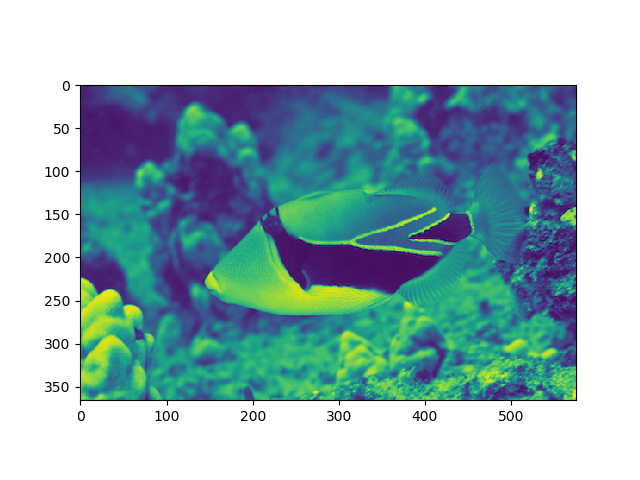
\includegraphics[width=\linewidth]{code/humu-color.png}
 \caption{Humu Color}
\label{label}

\end{figure}

\begin{figure}

\centering
  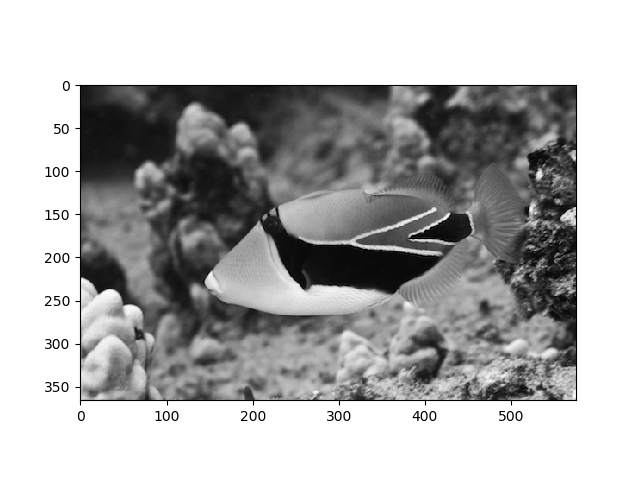
\includegraphics[width=\linewidth]{code/humu-gray.png}
 \caption{Humu Greyscale}
\label{label}

\end{figure}

\begin{figure}

\centering
  \includegraphics[width=\linewidth]{code/random.png}
 \caption{Random Image}
\label{label}

\end{figure}

\newpage

\textbf{PART B}

{\bf Solution.} 

\begin{verbatim}
$ cat -n walk.py
     1	#!/usr/bin/env python3
     2	
     3	"""
     4	walk.py - manipulate and plot "walk.txt"
     5	Ken Youens-Clark
     6	27 August 2018
     7	"""
     8	
     9	import numpy as np
    10	import matplotlib.pyplot as plt
    11	
    12	
    13	# --------------------------------------------------
    14	def main():
    15	    """
    16	    main()
    17	    """
    18	    dat = np.loadtxt('../data/walk.txt')
    19	    print('Data  : min "{:5}, max "{:5}", shape "{}"'.format(
    20	        dat.min(), dat.max(), dat.shape))
    21	
    22	    abs_min = np.abs(dat.min())
    23	    scaled = (dat + abs_min) / (dat.max() + abs_min)
    24	    print('Scaled: min "{:5}, max "{:5}", shape "{}"'.format(
    25	        scaled.min(), scaled.max(), scaled.shape))
    26	
    27	    outfile = '../data/walk_scale01.txt'
    28	    np.savetxt(outfile, scaled)
    29	    print('Scaled data saved to "{}"'.format(outfile))
    30	
    31	    plot_1d_array(arr=dat, title='Original', outfile='walk.png')
    32	    plot_1d_array(arr=scaled, title='Scaled', outfile='walk_scaled.png')
    33	
    34	
    35	# --------------------------------------------------
    36	def plot_1d_array(arr, title=None, outfile=None):
    37	    """
    38	    Plot a 1D array
    39	    :param: arr - a 1D Numpy array
    40	    :param: title - figure title (str)
    41	    :param: outfile - path to write image (str)
    42	
    43	    :return: void
    44	    """
    45	
    46	    plt.figure()
    47	    if title:
    48	        plt.title(title)
    49	    plt.plot(arr)
    50	
    51	    if outfile:
    52	        plt.savefig(outfile)
    53	        print('Wrote to "{}"'.format(outfile))
    54	
    55	    plt.show()
    56	
    57	
    58	# --------------------------------------------------
    59	if __name__ == '__main__':
    60	    main()
$ ./walk.py
Data  : min " -1.0, max "  5.0", shape "(200,)"
Scaled: min "  0.0, max "  1.0", shape "(200,)"
Scaled data saved to "../data/walk_scale01.txt"
Wrote to "walk.png"
Wrote to "walk_scaled.png"

\end{verbatim}

\begin{figure}
\centering
  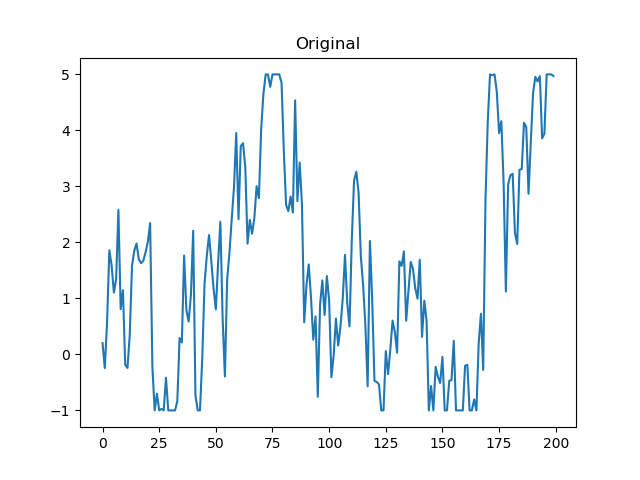
\includegraphics[width=\linewidth]{code/walk.png}
 \caption{Plot of original walk data}
\label{label}
\end{figure}

\begin{figure}
\centering
  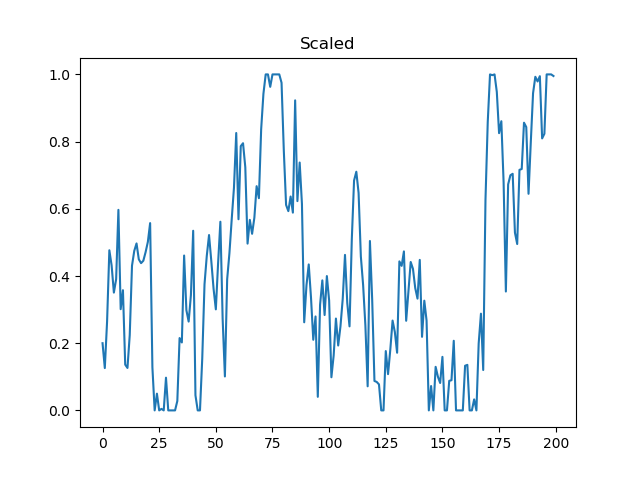
\includegraphics[width=\linewidth]{code/walk_scaled.png}
 \caption{Plot of scaled walk}
\label{label}
\end{figure}

\pagebreak

%%%   Problem 7
\item \label{prob:7} [1 point]
Functions:

{\bf Solution.} 

\begin{verbatim}

def main():
    """
    main
    :param: none
    :return: void
    """
    exercise6("../data/humu.txt", "out.txt")

def scale01(arr):
    """
    Linearly scale the values of an array in the range [0,1]
    :param arr: input ndarray
    :return: scaled ndarray
    """
    return arr / arr.max()
    
def exercise6(infile, outfile):
    """
    Read a file into a Numpy ndarray
    :param infile: the file to read
    :param outfile: where to write the output
    :return: void
    """
    dat = np.loadtxt(infile)

    scaled = scale01(dat)
    print('scaled min = {} max = {} shape = {}'.format(scaled.min(),
                                                       scaled.max(),
                                                       scaled.shape))

    plt.figure()
    plt.imshow(dat)
    plt.show()

    print(plt.cm.cmapname)

    plt.imshow(dat, cmap='gray')
    plt.show()

    for _ in range(0, 2):
        ran = np.random.random(dat.shape)
        plt.imshow(ran)
        plt.show()
        np.savetxt(outfile, ran)

    ran1 = np.loadtxt(outfile)
    plt.imshow(ran1)
    plt.show()

    print('Done.')

if __name__ == '__main__':
    main()

$ ./hw1.py
type = <class 'numpy.ndarray'>
size = 210816
shape = (366, 576)
max = 0.9450980392156862
min = 0.0
scaled min = 0.0 max = 1.0 shape = (366, 576)
tab20c_r
Done.

\end{verbatim}


%%%   Problem 8
\item \label{prob:8} [2 points]
Documenting:

\emph{Functions documented above}

%%%   Problem 9
\item \label{prob:9} [2 points]
Random Numbers:

{\bf Solution.} 

I wrote the following function:

\begin{verbatim}
def exercise9():
    """
    Estimate the randomness of throwing double-sixes
    :param: none
    :return: void
    """

    np.random.seed(seed=8)

    throws = 1000
    dbl6 = 0
    for _ in range(0, throws):
        (n1, n2) = np.random.randint(low=1, high=7, size=2, dtype=int)
        #print('{} {}'.format(n1, n2))
        if n1 == 6 and n2 == 6:
            dbl6 += 1

    print('Threw double-six {:.2}%'.format((dbl6 / throws) * 100))
\end{verbatim}

Everytime I run it, I get the same result, "2.6\%".

\begin{verbatim}
$ ./hw1.py
Threw double-six 2.6%
$ ./hw1.py
Threw double-six 2.6%
\end{verbatim}

If I comment out {\tt seed=8}, I will get different results:

\begin{verbatim}
$ for i in $(seq 1 9); do echo -n "$i: " && ./hw1.py; done
1: Threw double-six 2.7%
2: Threw double-six 2.4%
3: Threw double-six 3.4%
4: Threw double-six 2.1%
5: Threw double-six 2.6%
6: Threw double-six 2.6%
7: Threw double-six 2.3%
8: Threw double-six 3.2%
9: Threw double-six 3.2%
\end{verbatim}

Putting back in {\tt seed=8}, I go back to the same result:

\begin{verbatim}
$ for i in $(seq 1 10); do echo -n "$i: " && ./hw1.py; done
1: Threw double-six 2.6%
2: Threw double-six 2.6%
3: Threw double-six 2.6%
4: Threw double-six 2.6%
5: Threw double-six 2.6%
6: Threw double-six 2.6%
7: Threw double-six 2.6%
8: Threw double-six 2.6%
9: Threw double-six 2.6%
10: Threw double-six 2.6%
\end{verbatim}

\emph{Explain why it is often important to have random number sequences that are not really random, and can be controlled}

Being able to count on a "random" number allows one to write tests for such functions.

\emph{The generation of random numbers is too important to be left to chance.} -- Robert R. Coveyou

%%%   Problem 10
\item \label{prob:10} [5 points] Random Numbers, Vectors, Matrices, and Operations

{\bf Solution~\ref{prob:10}a.} 

\begin{verbatim}
def exercise10a():
    """
    Print two three-dimensional column vectors
    :param: none
    :return: void
    """

    np.random.seed(seed=5)
    a = np.random.rand(3, 1)
    b = np.random.rand(3, 1)
    print(a)
    print(b)
    
$ ./hw1.py
[[0.22199317]
 [0.87073231]
 [0.20671916]]
[[0.91861091]
 [0.48841119]
 [0.61174386]]
\end{verbatim}

{\bf Solution~\ref{prob:10}b.} 

\begin{verbatim}
def exercise10b():
    """
    Print two three-dimensional column vectors
    :param: none
    :return: void
    """

    np.random.seed(seed=5)
    a = np.random.rand(3, 1)
    b = np.random.rand(3, 1)
    print("a\n {}".format(a))
    print("b\n{}".format(b))
    print("a + b\n{}".format(a + b))
    print("a * b\n{}".format(a * b))
    print("aT . b\n{}".format(a.transpose().dot(b)))

a
 [[0.22199317]
 [0.87073231]
 [0.20671916]]
b
[[0.91861091]
 [0.48841119]
 [0.61174386]]
a + b
[[1.14060408]
 [1.35914349]
 [0.81846302]]
a * b
[[0.20392535]
 [0.4252754 ]
 [0.12645917]]
aT . b
[[0.75565992]]
\end{verbatim}

\begin{equation}
\begin{aligned} 
  \mathbf{a} &= 
  \begin{bmatrix}
  0.22199317 & 0.87073231 & 0.20671916
  \end{bmatrix}
  \\
  \mathbf{b} &= 
  \begin{bmatrix}
  0.91861091 & 0.48841119 & 0.61174386
  \end{bmatrix}
  \\
  \mathbf{a} + \mathbf{b} &= 
  \begin{bmatrix}
  1.14060408 & 1.35914349 & 0.81846302
  \end{bmatrix}
  \\
  \mathbf{a} \circ \mathbf{b} &=
  \begin{bmatrix}
  0.20392535 & 0.4252754 & 0.12645917
  \end{bmatrix}
  \\
  \mathbf{a}^\top \mathbf{b} &= 0.75565992
\end{aligned}
\end{equation}


{\bf Solution~\ref{prob:10}c.} 

\begin{verbatim}
def exercise10c():
    """
    Vector/matrix manipulation
    :param: none
    :return: void
    """

    np.random.seed(seed=5)
    a = np.random.rand(3, 1)
    b = np.random.rand(3, 1)

    np.random.seed(seed=2)
    X = np.asmatrix(np.random.rand(3, 3))

    print("a\n {}".format(a))
    print("b\n{}".format(b))
    print("X\n{}".format(X))
    print("aTX\n{}".format(a.transpose() * X))
    print("aTXb\n{}".format(a.transpose() * X * b))
    print("X-1\n{}".format(X.getI()))
a
 [[0.22199317]
 [0.87073231]
 [0.20671916]]
b
[[0.91861091]
 [0.48841119]
 [0.61174386]]
X
[[0.4359949  0.02592623 0.54966248]
 [0.43532239 0.4203678  0.33033482]
 [0.20464863 0.61927097 0.29965467]]
aTX
[[0.51814195 0.49979844 0.47159888]]
aTXb
[[1.00857572]]
X-1
[[-1.20936675  5.11771977 -3.42333228]
 [-0.96691719  0.279414    1.46561347]
 [ 2.82418088 -4.07257903  2.64627411]]
\end{verbatim}

\begin{equation}
\begin{aligned}
  \mathbf{a} &=
  \begin{bmatrix}
	0.22199317 & 0.87073231 & 0.20671916
  \end{bmatrix}
  \\
  \mathbf{b} &=
  \begin{bmatrix}
    0.91861091 & 0.48841119 & 0.61174386
  \end{bmatrix}
  \\
  \mathbf{X} &=
  \begin{bmatrix}
    0.4359949  & 0.02592623 & 0.54966248 \\
    0.43532239 & 0.4203678  & 0.33033482 \\
    0.20464863 & 0.61927097 & 0.29965467 \\
  \end{bmatrix}
  \\
  \mathbf{a}^\top\mathbf{X} &=
  \begin{bmatrix}
    0.51814195 & 0.49979844 & 0.47159888
  \end{bmatrix}
  \\
  \mathbf{a}^\top\mathbf{X}\mathbf{b} &= 1.00857572
  \\
  \mathbf{X}^{-1} &=
  \begin{bmatrix}
     1.20936675  &  5.11771977  & -3.42333228 \\
    -0.96691719  &  0.279414    &  1.46561347 \\
     2.82418088  & -4.07257903  &  2.64627411 \\
  \end{bmatrix}
\end{aligned}
\end{equation}

\pagebreak

%%%   Problem 11
\item \label{prob:11} [3 points] Simple Plotting


{\bf Solution11a.} 

\begin{figure}

\centering
  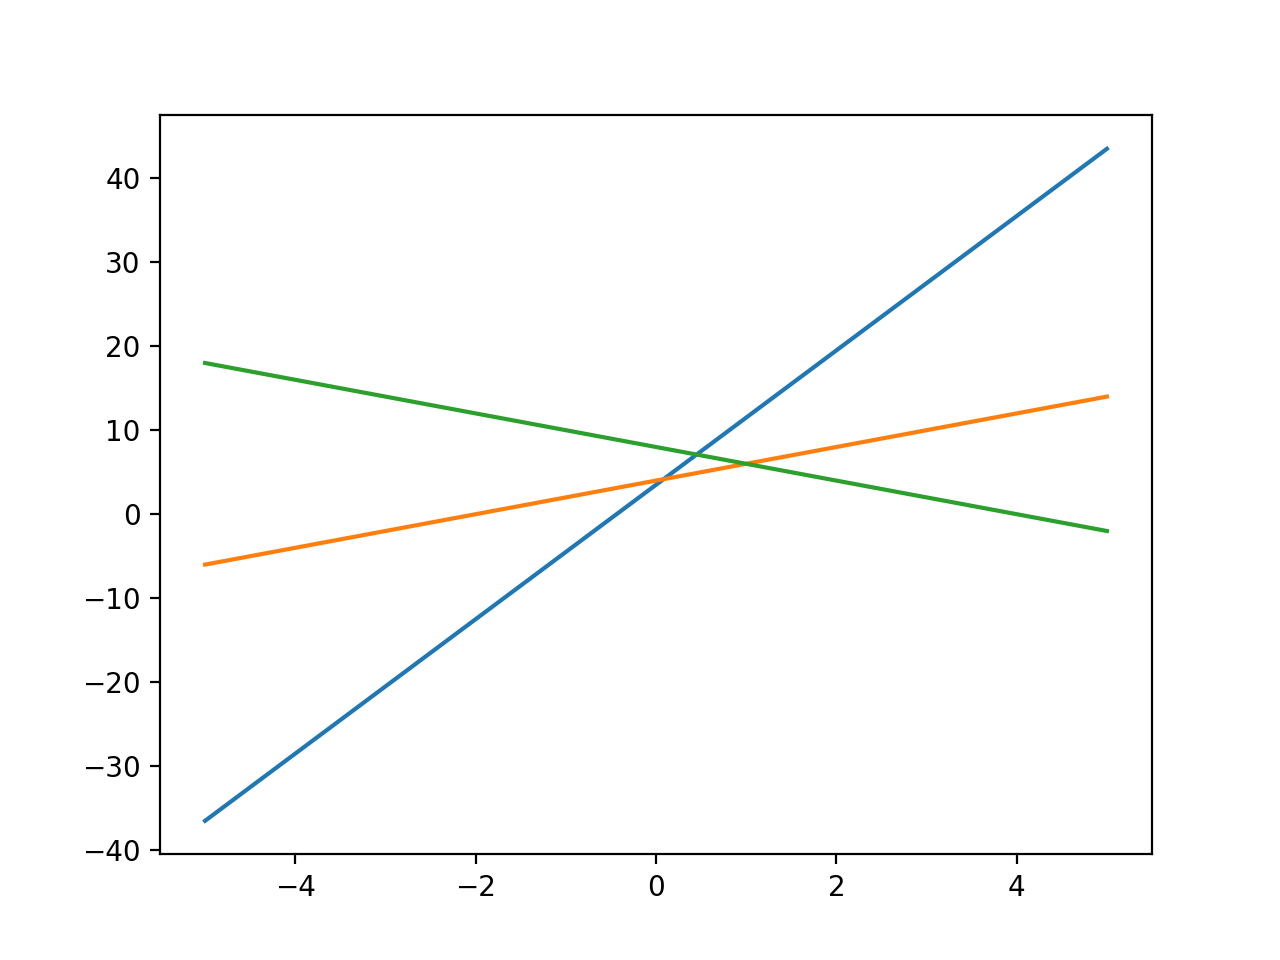
\includegraphics[width=\linewidth]{Figure_1.png}
 \caption{y = 3.5 + 8.0x; y = 4.0 + 2.0x; y = 8.0 + -2.0x}
\label{label}

\end{figure}

\begin{equation}
\begin{gathered}
y = 3.5 + 8.0x \\
y = 4.0 + 2.0x \\
y = 8.0 + -2.0x \\
\end{gathered}
\end{equation}

{\bf Solution11b.} 

\begin{figure}

\centering
  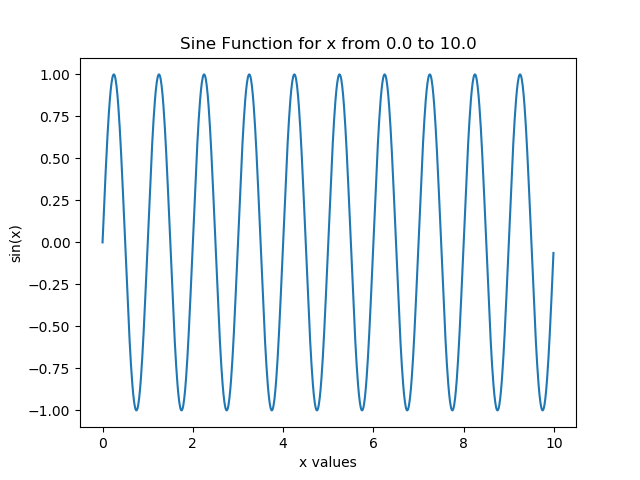
\includegraphics[width=\linewidth]{code/sine.png}
 \caption{Plot sin(x)}
\label{label}

\end{figure}

\begin{verbatim}
def exercise11():
    """
    Plotting
    :param: none
    :return: void
    """

    x = np.arange(0, 10, .01)
    y = np.sin(2 * np.pi * x)
    plt.plot(x, y)
    plt.title('Sine Function for x from 0.0 to 10.0')
    plt.xlabel('x values')
    plt.ylabel('sin(x)')
    plt.show()
    plt.savefig('sine.png')
\end{verbatim}




\end{enumerate}

\end{document}

